\section{Лекция 14 от 17.01.2017 \\ Метрические, нормированные и евклидовы пространства}

\subsection{Метрические пространства}

\begin{Def}
Метрическое пространство --- это упорядоченная пара $(M,\ \rho)$, где $M$ --- непустое множество, а $\rho:\ M\times M \to \R$ --- функция, называемая метрикой, которая удовлетворяет следующим свойствам:
\begin{enumerate}
\item $\forall x, y \in M\ \rho(x, y) \geq 0,$ причем $\rho(x, y) = 0 \Leftrightarrow x = y$;
\item $\forall x, y \in M\ \rho(x, y) = \rho(y, x)$;
\item $\forall x, y, z \in M\ \rho(x, y) \leq \rho(x, z) + \rho(z, y)$.
\end{enumerate}
\end{Def}

\begin{Examples}
Дискретная метрика (<<метрика ленивого человека>>):
$$
\rho(x, y) = \begin{cases}
0, & x = y;\\
1, & x \neq y.
\end{cases}
$$
\end{Examples}

Часто, когда говорят о метрических пространствах, называют только множество $M$, считая, что метрика подразумевается.

Пусть $\{x_n\}_{n=1}^{\infty}$ --- последовательность точек метрического пространства $M$.
\begin{Def}
$x_n \ito x $, $x\in M$, если $\rho(x_n, x) \ito 0$ или, что эквивалентно,
$$
\forall \eps > 0\ \exists N \in \N\ \forall n > N\ \rho(x_n, x) < \eps.
$$
\end{Def}

\begin{Statement}
Если $x_n \ito x$ и $x_n \ito \widetilde{x}$, то $x = \widetilde{x}$.
\end{Statement}
\begin{proof}
Вспомним, что $\rho(x, \widetilde{x}) \leq \rho(x, x_n) + \rho(x_n, \widetilde{x})$. Тогда при $n \to \infty$ получаем, что $0 \leq \rho(x, \widetilde{x}) \leq 0$, то есть $\rho(x, \widetilde{x}) = 0$, что и означает их равенство. 
\end{proof}

В силу отсутствия арифметических операций над элементами произвольных метрических пространств, никаких арифметических свойств предела тут не может быть (<<это как складывать или делить стулья>>).

А вот критерий Коши есть.
\begin{Def}
Последовательность $\{x_n\}_{n=1}^\infty$ метрического пространства называется фундаментальной (последовательностью Коши, удовлетворяющей условию Коши), если
$$
\forall \eps > 0 \ \exists N \in \N\ \forall n, m > N\ \rho(x_n, x_m) < \eps.
$$
\end{Def}
\begin{Statement}
	Если последовательность точек метрического пространства сходится, то она фундаментальна.
\end{Statement}
\begin{proof}
	 Как всегда, через $\eps/2$ и неравенство треугольника.
\end{proof}
Хочется сказать как обычно: последовательность имеет предел тогда и только тогда, когда она фундаментальная. Но вот проблема --- это неверное утверждение. Несложный пример: $M = \R\setminus\{0\}$ и $x_n = 1/n$. Эта последовательность вроде как должна сходиться к нулю, вот только его нет в нашем пространстве, так что в итоге последовательность не сходится.

Но критерий Коши крайне важная вещь, без него ломается куча теорем, поэтому хочется его все-таки иметь. Для этого наложим дополнительное требование на наши метрические пространства.
\begin{Def}
Метрическое пространство называется полным, если в нем каждая последовательность Коши имеет предел.
\end{Def}

\begin{Theorem}[Критерий Коши]
Последовательность $\{x_n\}_{n=1}^\infty$ точек полного метрического пространства сходится тогда и только тогда, когда эта последовательность фундаментальна.
\end{Theorem}

\begin{Comment}
Шутки ради. Из \href{https://goo.gl/drRQz0}{теоремы Бэра} можно получить следствие, которое с точки зрения русского языка звучит прекрасно: полное пространство не может быть тощим.
\end{Comment}

\subsection{Шары в метрическом пространстве}
В метрическом пространстве естественным образом возникают фигуры.
\begin{Def}\ 
\begin{enumerate}
\item Открытый шар: $B_r(x_0) = \{x \in M \mid \rho(x, x_0) < r  \}$.
\item Закрытый шар: $\overline{B}_r(x_0) = \{x \in M \mid \rho(x, x_0) \leq r  \}$.
\end{enumerate}
\end{Def}

Вообще говоря, эти шары совершенно не обязательно должны быть как-то похожи на шары в привычном нам понимании. В качестве иллюстрации приведем два примера.
\begin{Examples}
Пусть $M = \N$. Рассмотрим две метрики: $\rho(m, n) = 1 + \dfrac{1}{\min(n, m)}$ и $\widetilde{\rho}(m, n) = 1 + \dfrac{1}{\max(n, m)}$, если $n \neq m$, иначе 0. Это действительно метрики, как несложно убедиться.

Рассмотрим закрытый шар $\overline{B}_{1 + 1/n}(n)$. В метрике $\rho$ он задает множество $\{n, n+1, n+2, \ldots\}$, а в метрике $\widetilde{\rho}$ --- все $\N$. 
\end{Examples}

\begin{Examples}
А может ли шар большего радиуса строго включаться в шар меньшего радиуса? Да, причем это даже довольно несложно нарисовать.

Пусть $M$ --- это шар единичного радиуса в пространстве $\R^2$. Возьмем точку, близкую к окружности, и построим шар радиуса $1.5$ с центром в этой точке. Он не влезет полностью в наше пространство, за счет чего мы и получим строгое включение его в шар меньшего радиуса.
\begin{figure}[H]
\center{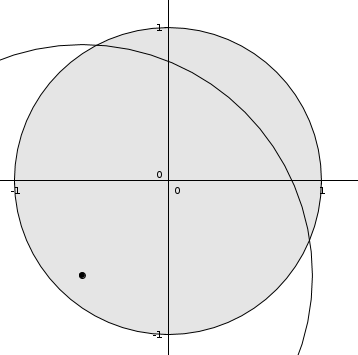
\includegraphics[width=0.35\linewidth]{14-1} }
\caption{Заштрихованная часть соответствует множеству $M$}
\end{figure}
\end{Examples}

\subsection{Нормированные пространства}
Все это конечно замечательно, но хочется, чтобы метрика как-то согласовывалась с пространством, а то иначе неинтересно получается.

\begin{Def}
Нормированное пространство --- это упорядоченная пара $(L, ||.||)$, где $L$ --- линейное пространство, а $||.||:\ L \to \R$ --- функция, называется нормой, которая удовлетворяет следующим свойствам:
\begin{enumerate}
\item $\forall x \in L\ ||x|| \geq 0$, причем $||x|| = 0 \Leftrightarrow x = 0$;
\item $\forall x \in L\ \forall \alpha \in \R\ ||\alpha x|| = |\alpha|\cdot ||x||$;
\item $\forall x, y \in L\ ||x + y|| \leq ||x|| + ||y||$.
\end{enumerate}
\end{Def}

\begin{Statement}
Норма порождает метрику $\rho(x, y) = ||x - y||$. Это действительно метрика, как несложно убедиться, и по умолчанию нормированные пространства рассматриваются как метрические с данной метрикой.
\end{Statement}

\begin{Comment}
Обратное неверно: не любая метрика порождена какой-то нормой! Например, дискретная метрика.
\end{Comment}

И да, нормированные пространства тоже бывают неполными. Здесь, правда, уже не найдется очевидного примера, потому что так просто из линейного пространства одну точку не выколоть. Так что пока верьте на слово.
\begin{Def}
Полные нормированные пространства называются Банаховыми.
\end{Def}

Нормы бывают какими угодно. Например, в классической декартовой системе, где $v = (x, y)$, обычно рассматривают следующие нормы:
\begin{itemize}
\item $||v|| = ||v||_1 = |x| + |y|$ --- манхэттенская норма, $l_1$--норма;
\item $||v|| = ||v||_2 = \sqrt{x^2 + y^2}$ --- евклидова норма, $l_2$--норма;
\item $||v|| = ||v||_\infty = \max(|x|, |y|)$ --- <<бесконечная норма>>.
\end{itemize}

Вообще говоря, это частные случаи $p$--норм: $||v||_p = (|x|^p + |y|^p)^{1/p}$. Но на практике $p$--нормы, где $p$ отлично от 1 и 2 не встречаются (за исключением <<бесконечной нормы>>).

Ниже приведено, как выглядят единичные шары в разных нормах.
\begin{figure}[H]
\begin{minipage}[h]{0.47\linewidth}
\center{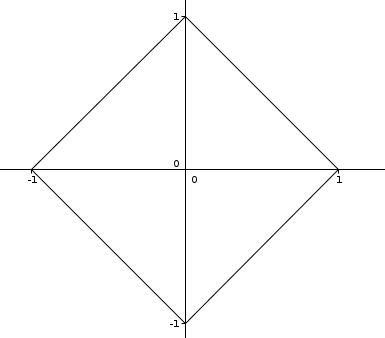
\includegraphics[width=0.6\linewidth]{14-2} 
    \caption{Манхэттенская норма}}
\end{minipage}
\hfill
\begin{minipage}[h]{0.47\linewidth}
\center{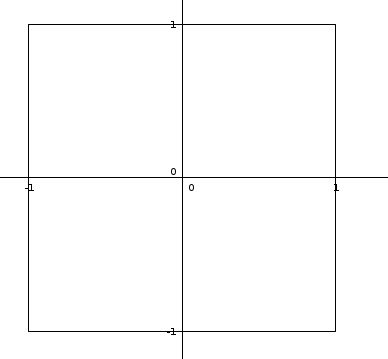
\includegraphics[width=0.6\linewidth]{14-3} 
    \caption{Бесконечная норма}}
\end{minipage}
\end{figure}

\begin{Task}[Бонусная задача]
Рассмотрим плоскость, $\R^2$. Константу $\pi$ можно воспринимать как половину длины единичной окружности: $\pi = l/2$. Но вообще говоря, в зависимости от выбранной нормы, единичная окружность имеет разный вид и, соответственно, длину. Например, в нормированном пространстве с бесконечной нормой $l = 8$, и тогда $\pi = 4$. Как мы видим, константа $\pi$ разная для разных нормированных пространств над множеством $\R^2$.

Доказать, что для любой нормы на плоскости $3 \leq \pi \leq 4$, причем оценка не улучшаема.
\end{Task}

\subsection{Евклидовы пространства}
Норма тоже бывает не сама по себе, она может быть порождена скалярным произведением.
\begin{Def}
Евклидово пространство --- это упорядоченная пара $(L, (., .))$, где $L$ --- линейное пространство над $\R$, а $(., .):\ L\times L \to \R$ --- функция, называемая скалярным произведением, которая удовлетворяет следующим свойствам:
\begin{enumerate}
\item $\forall x \in L\ (x, x) \geq 0$, причем $(x, x) = 0 \Leftrightarrow x = 0$;
\item $\forall x, y\in L\ (x, y) = (y, x)$;
\item $\forall x_1, x_2, y \in L,\ \forall \alpha_1, \alpha_2 \in \R\ (\alpha_1x_1 + \alpha_2x_2, y) = \alpha_1(x_1, y) + \alpha_2(x_2, y)$.
\end{enumerate}
Иными словами, это билинейная симметричная положительно определенная функция.
\end{Def}

\begin{Examples}
$L = C[a, b]$, $(f, g) = \int\limits_a^bf(x)g(x)\mathrm{d}x$ --- бесконечномерное евклидово пространство.
\end{Examples}

\begin{Theorem}[Неравенство Коши-Буняковского-Шварца]
Пусть $(L, (., .))$ --- евклидово пространство. Тогда $\forall x, y \in L$ верно, что $|(x, y)| \leq \sqrt{(x, x)}\cdot\sqrt{(y, y)}$, причем равенство имеет место тогда и только тогда, когда $x$ и $y$ линейно зависимы.
\end{Theorem}
Доказательство будет на следующей лекции.

\begin{Statement}
Скалярное произведение задает норму $||x|| = \sqrt{(x, x)}$. Несложно убедиться, что это действительно норма.
\end{Statement}
